We first measure the effect in isolation, on a corpus built so that the number of
aspects per document is a controlled variable.

\paragraph{Construction.}
Each document concatenates $k$ passages drawn from $k$ of ten mutually unrelated
topic pools. Every passage realises one \emph{fact}, a (pool, attribute, action)
triple, and a query asks about one fact in wording that shares no template with
the passages. Relevance is therefore defined by the generative process rather
than assumed: every document carrying a passage that realises the queried fact is
relevant, which yields relevance sets of 3.7 documents per query at $k=1$ rising
to 33.3 at $k=10$. Two representations of the same document are compared: one
pooled embedding of the whole text, and $k$ per-aspect embeddings scored by their
maximum. Both are scored at document level. We use 500 documents and 200 queries
per setting, encoder \texttt{all-MiniLM-L6-v2}, seed 13.

\paragraph{Result.}
Table~\ref{tab:dilution} and Figure~\ref{fig:dilution} report the outcome. The
per-aspect representation holds its similarity to relevant documents almost
exactly constant as $k$ grows, from 0.498 at $k=1$ to 0.493 at $k=10$, while the
pooled representation decays monotonically to 0.235. Retrieval follows: the
pooled system loses more than half its nDCG@10 between $k=1$ and $k=2$ and does
not recover, while the card system stays between 0.556 and 0.682 throughout. At
$k=1$ the two systems are identical by construction, and the measurement confirms
it exactly, which is a useful check on the pipeline.

\begin{table}[t]
\caption{Aspect dilution. Deltas are per-query paired differences,
card system minus pooled, with 95\% bootstrap intervals and paired permutation
$p$-values Holm-corrected across all 21 comparisons. Relevance-set sizes grow
with $k$ by construction, so nDCG is comparable down a column and between the two
systems within a row, but not across rows.}
\label{tab:dilution}
\centering
\begin{tabular}{rrrrrl}
\toprule
$k$ & pooled & cards & $\Delta$ & 95\% CI & win/tie/loss \\
\midrule
1  & 0.682 & 0.682 & $+0.000$ & exact tie & 0/200/0 \\
2  & 0.395 & 0.571 & $+0.177$ & $[+0.145, +0.207]$ & 160/0/40 \\
3  & 0.308 & 0.565 & $+0.257$ & $[+0.226, +0.288]$ & 173/1/26 \\
4  & 0.271 & 0.556 & $+0.285$ & $[+0.253, +0.317]$ & 175/0/25 \\
5  & 0.300 & 0.585 & $+0.285$ & $[+0.251, +0.318]$ & 176/2/22 \\
7  & 0.282 & 0.656 & $+0.374$ & $[+0.339, +0.408]$ & 182/0/18 \\
10 & 0.273 & 0.672 & $+0.399$ & $[+0.360, +0.438]$ & 186/1/13 \\
\bottomrule
\end{tabular}
\end{table}

\begin{figure}[t]
\centering
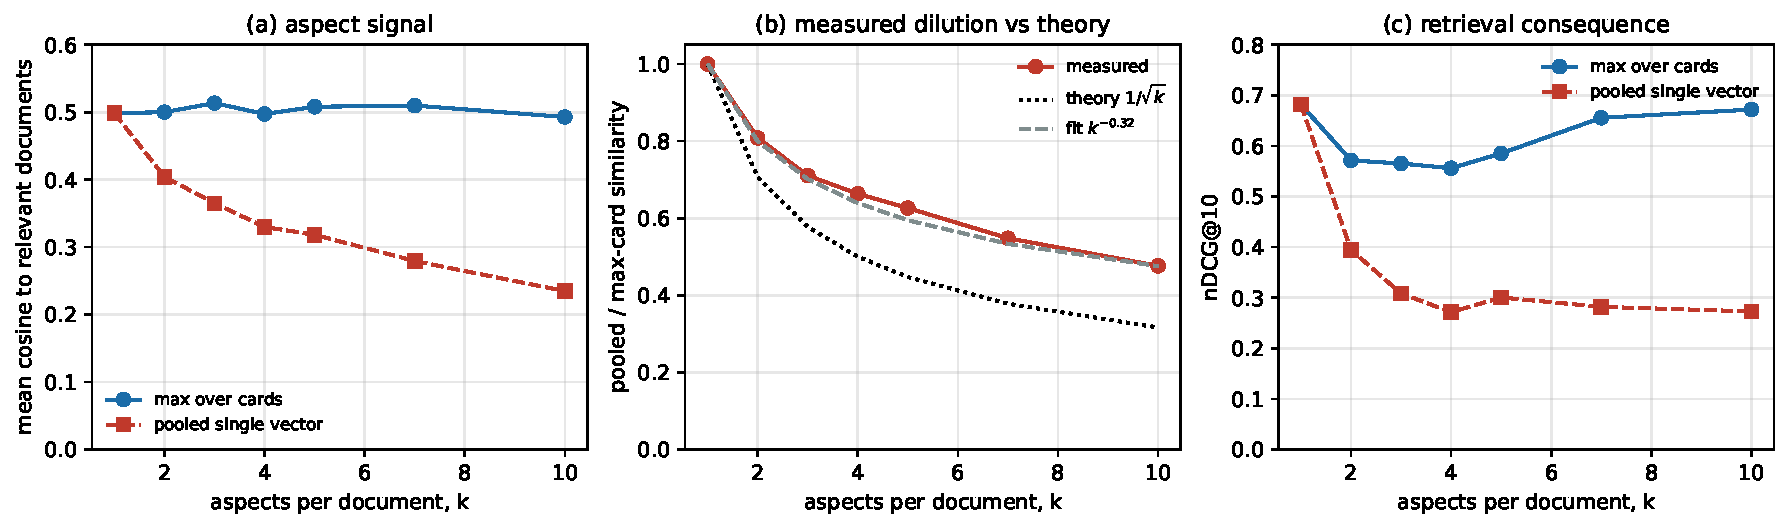
\includegraphics[width=\textwidth]{figures/fig1_dilution.pdf}
\caption{Aspect dilution as a function of $k$. Left: the aspect signal is
preserved by cards and lost by pooling. Centre: measured dilution against the
$1/\sqrt{k}$ prediction and a fitted power law. Right: the retrieval
consequence.}
\label{fig:dilution}
\end{figure}

\paragraph{The theory has the right shape and the wrong magnitude.}
Treating a pooled vector as the normalised mean of $k$ near-orthogonal aspect
vectors predicts that an aspect-directed query's similarity falls as
$1/\sqrt{k}$. The measured ratio of pooled to card similarity instead follows
$k^{-0.32}$, well above the prediction at every $k$. Two properties of real
encoders explain the gap, and both work in the same direction: aspects drawn from
natural language are not orthogonal, since all of the passages share register and
syntax, and encoder similarities are anisotropic, occupying a narrow cone that
compresses differences. We therefore report the orthogonality argument as an
upper bound on dilution rather than as a prediction that the data confirm.
